\chapter{Theory}
\label{ch:theory}

\emph{Write an intro to the chapter}.

\section{Instruments}
\label{theory:instruments}

The data in this project was acquired in an SEM with an EDS detector, which both are described in this section.


\subsection{SEM}
\label{theory:instruments:sem}

This subsection about SEM is based on Goldstein \cite{goldstein_scanning_2018}.

Scanning electron microscopes provide a high spatial resolution of micro- and nanoscale features.
The features revealed can be size, composition, shapes, topology, crystallography, and other chemical and physical properties. % Kinda copied from Goldstein p. VII
The working principle of an SEM is based on the interaction of a finely focused beam of electrons with the sample, where the beam is scanned over the sample surface to create a 2D image.
The interactions between the beam and the sample produce multiple signals, both as electrons and photons, which provide different information about the sample.
Auger electrons and secondary electrons give information about the surface of the sample, while backscattered electrons and X-rays give information about the composition of the sample.
The signals are not only created at the surface, but also inside the sample, and the region where the signals are created is called the interaction volume.

% The inteaction volume
After the interaction and creation of a signal, the signal must escape the sample to be registered by a detector.
The escape depth of the signal types is illustrated in \cref{fig:interaction_volume}.
When a signal is formed inside the sample, the signal can both be absorbed or scattered within the sample.
The signals with low energy are absorbed, and will thus only be emitted at the surface, e.g. Auger electrons and secondary electrons.
The signals which originate from deeper inside the sample, e.g. backscattered electrons and X-rays, can interact with the sample multiple times before they are emitted and detected.

% add typical depth for X-rays, cite eg. Hollas


% figures/interaction_volume.png
\begin{figure}[ht]
    \centering
    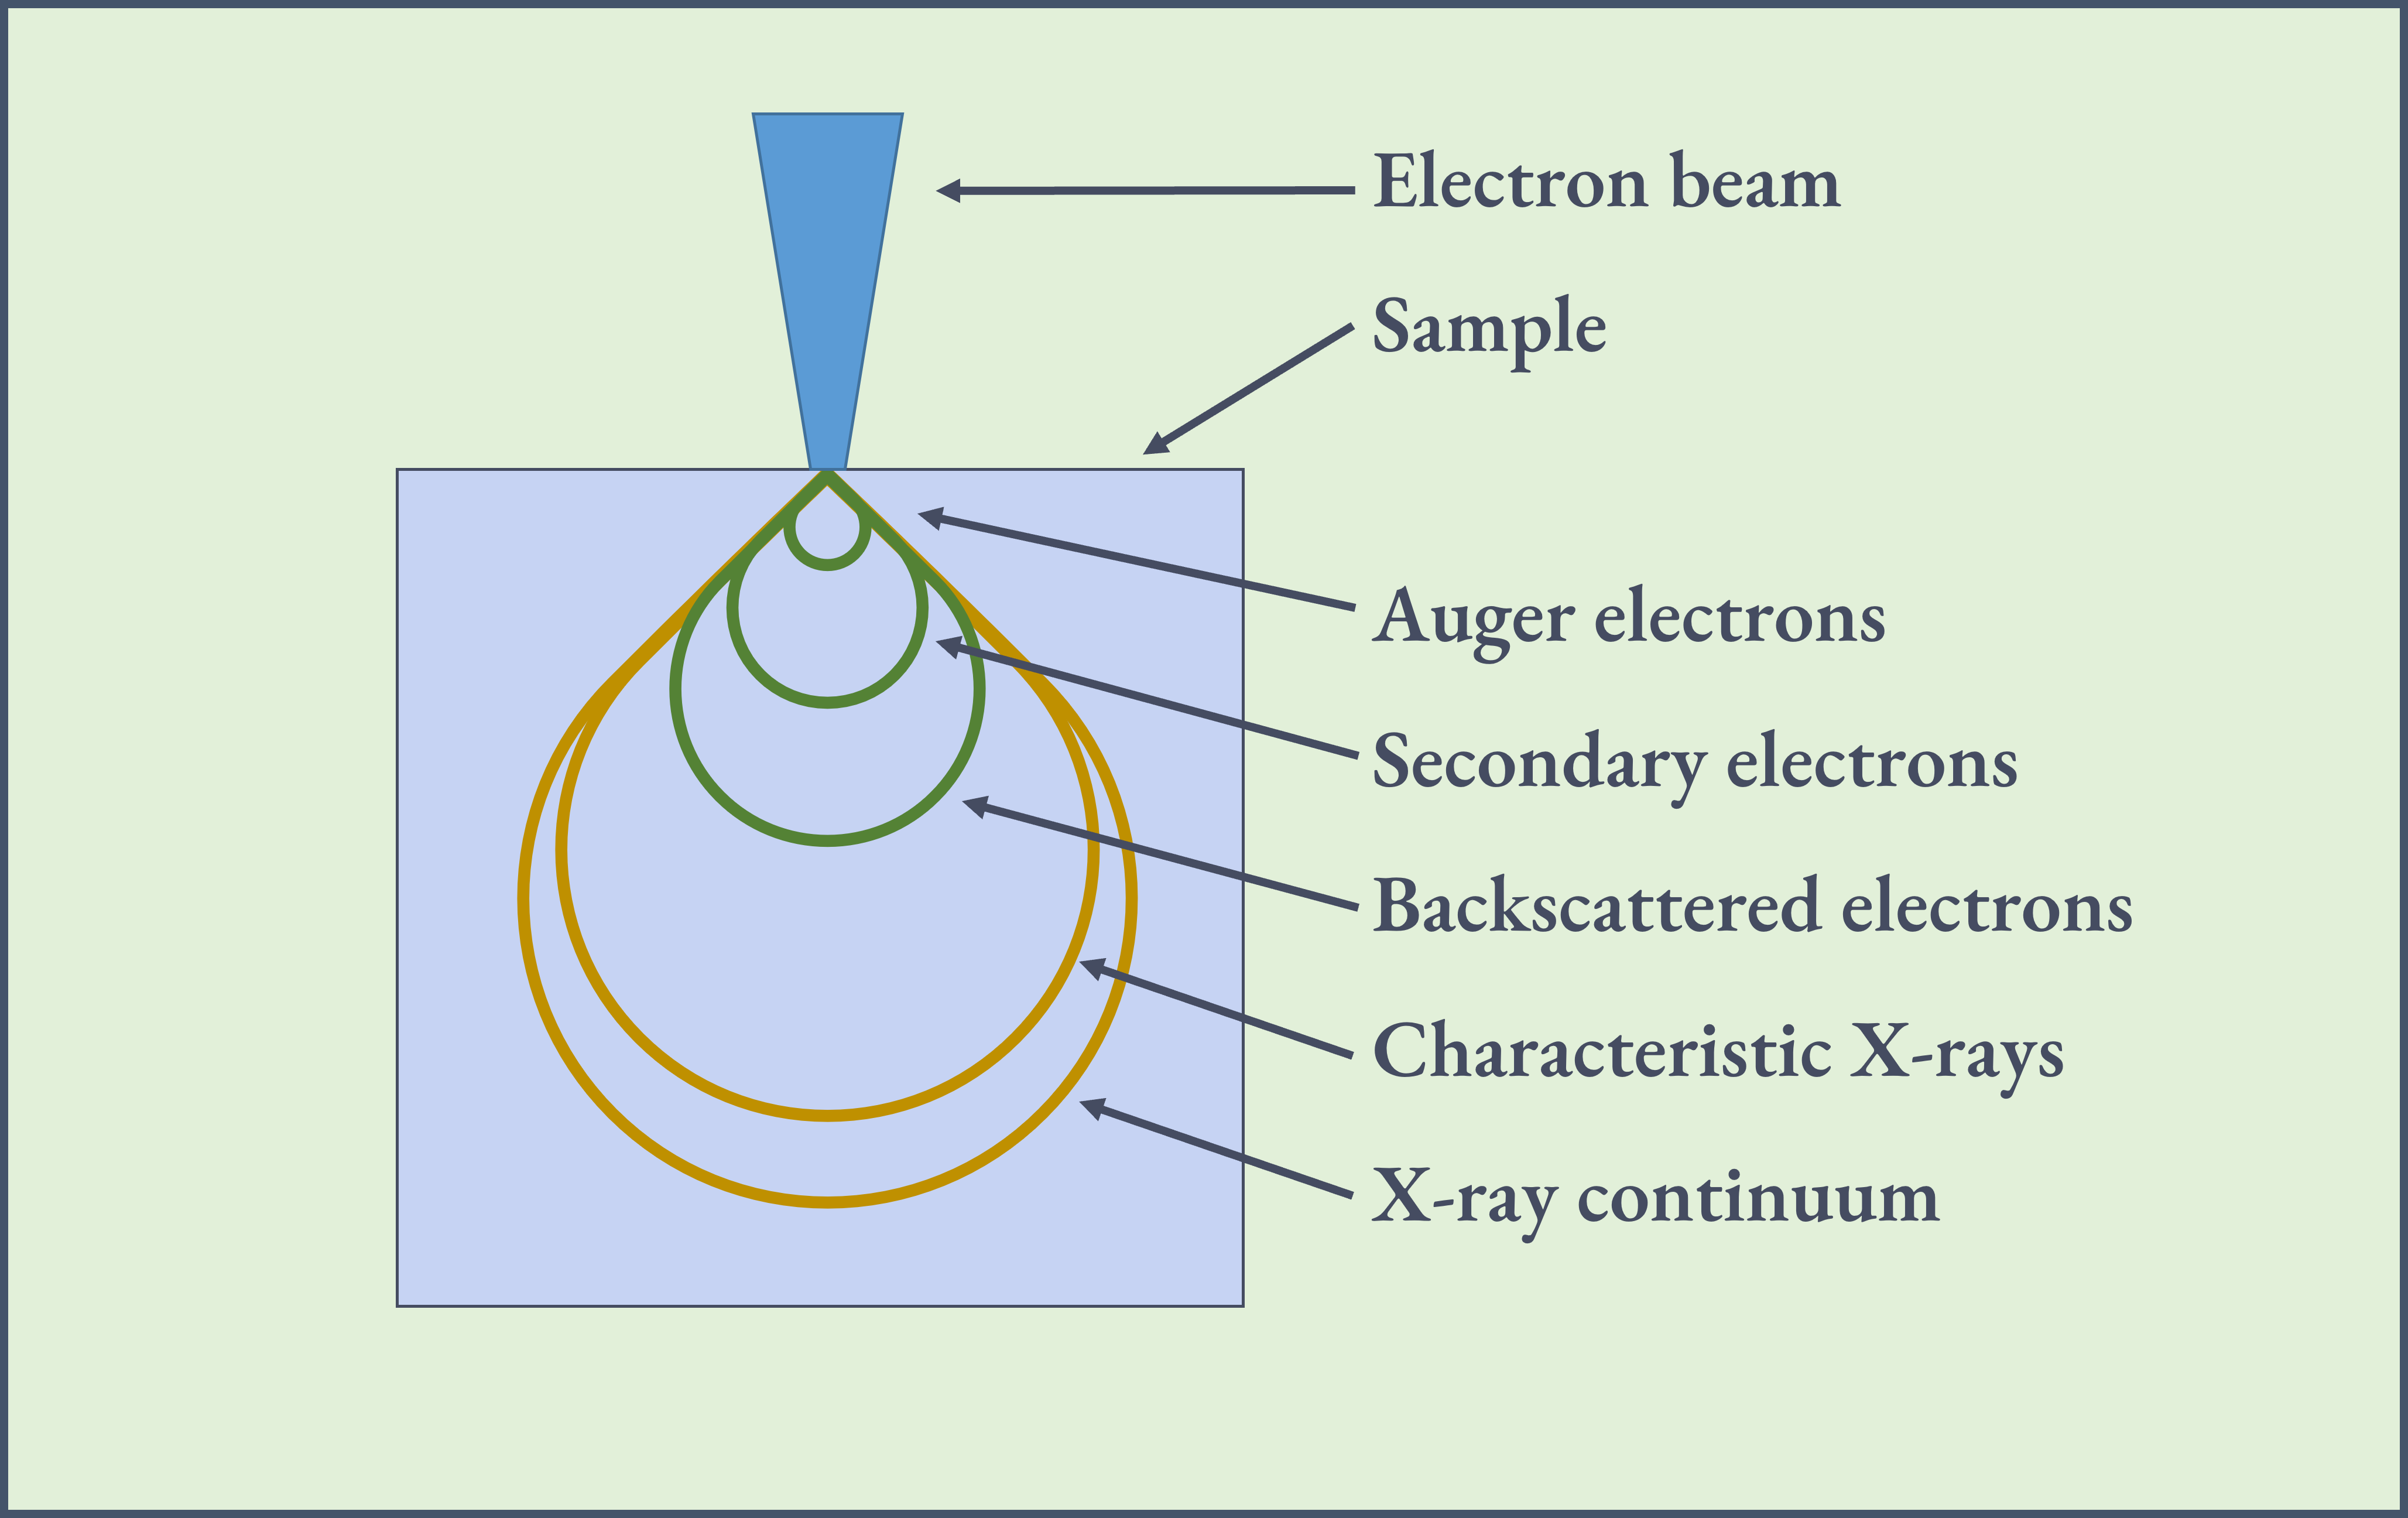
\includegraphics[width=0.8\linewidth]{figures/interaction_volume.png}
    \caption{
        Illustration of the interaction volume of the different signals.
        The signals are emitted in all directions, which is why the interaction volume is spherical.
        The blue signals are electrons and the orange signals are X-rays.
        The depths are not to scale.
        \brynjar{Add depth ranges?}
    }
    \label{fig:interaction_volume}
\end{figure}


% \ton{Do you want me to write about the different signals, ie. SE and BSE?}


% The parts in the SEM
An SEM consists of several parts, which are illustrated in \cref{fig:SEM_setup}.
The electron gun is the source of the electrons.
The condenser lens focuses the electrons to a small beam.
The two apertures sets the size of the beam, which is important since the electrons closest to the central axis of the beam have the fewest aberrations.
The scanning coils are used to scan the beam over the sample in the raster fashion.
The objective lens focuses the beam to a small spot on the sample.
In general a smaller spot allows higher resolution, because the signal is recorded from a smaller area.
However, this effect is limited by several factors, such as the interaction volume.
The detectors are placed above the sample.

% \ton{What more do you want me to write about the SEM?}

% figure/SEM_setup.png
\begin{figure}[ht]
    \centering
    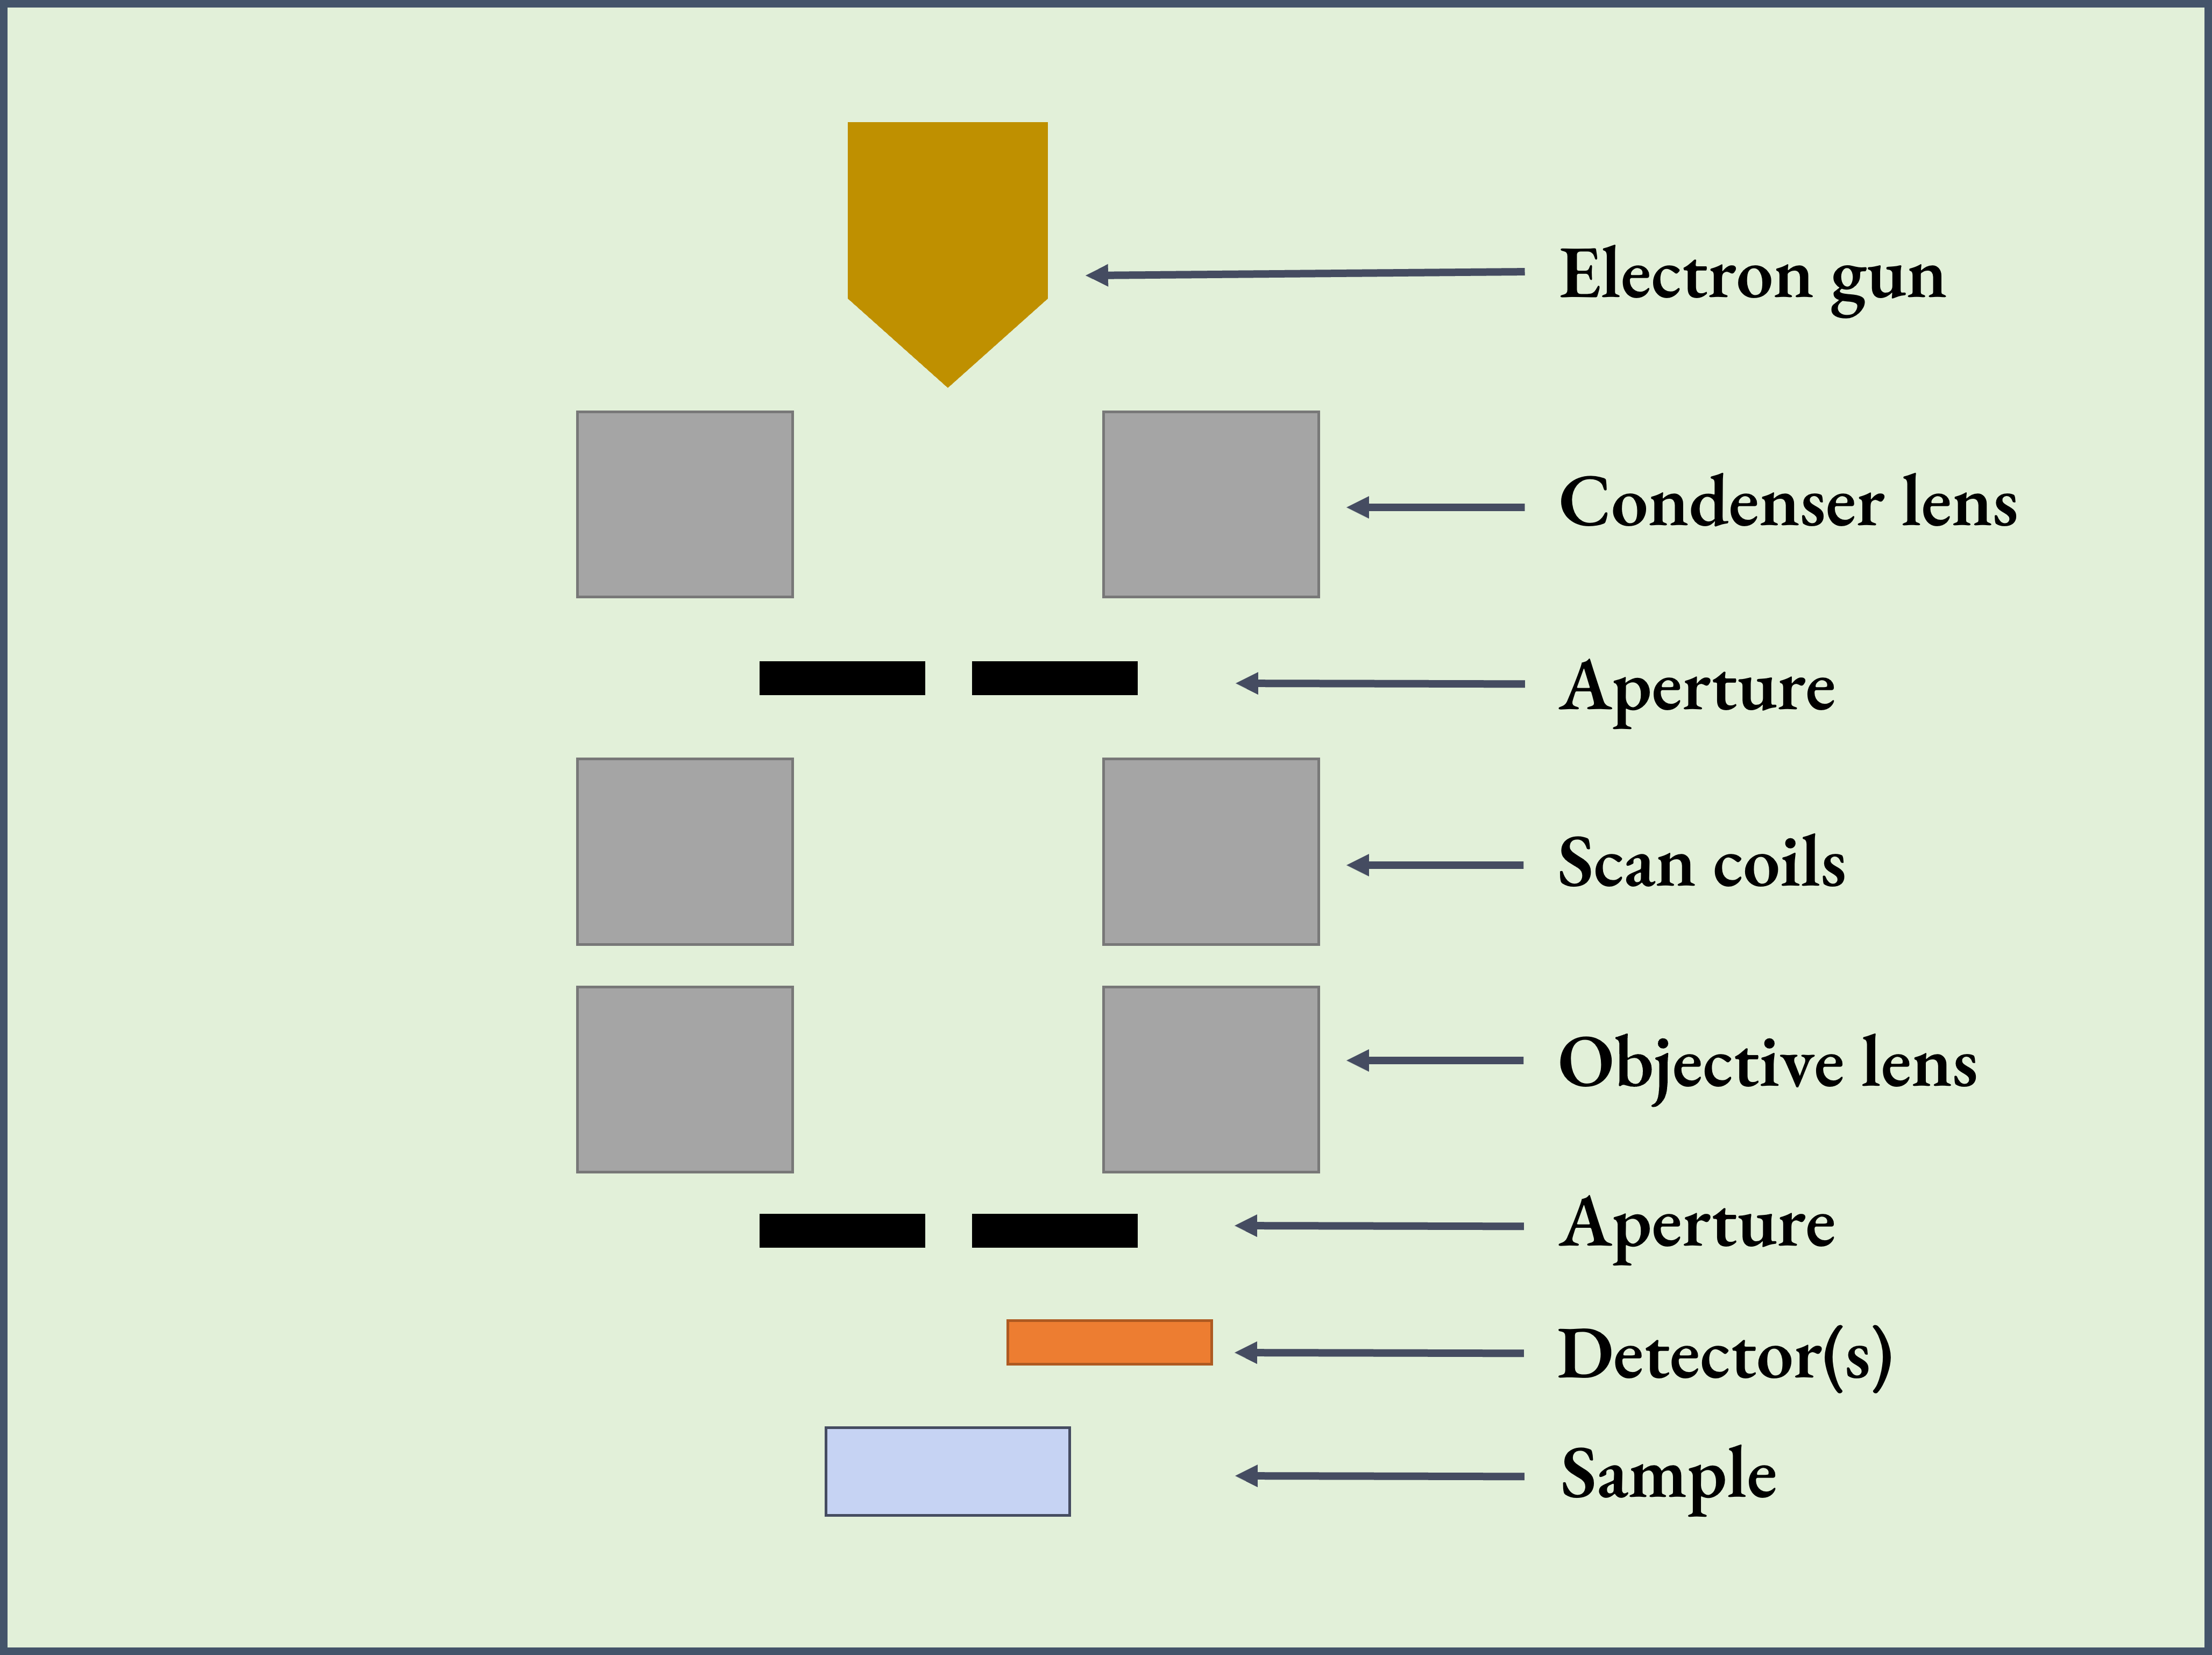
\includegraphics[width=0.8\linewidth]{figures/SEM_setup.png}
    \caption{
        Illustration of the parts in an SEM.
    }
    \label{fig:SEM_setup}
\end{figure}















\subsection{The EDS system}

The EDS system is made up of the detector, the electronics, and the software on the computer.
Traditionally, the EDS detector have been a Si(Li) detector, but now the most common detector is a silicon drift detector (SDD).
An overview of the two detectors is given below.
Both detectors are Si based diode-structures, which have different structures, but the same a three-step process for the detection of X-rays.
% detecting X-rays
First an incoming X-ray is absorbed in the detector, which ionizes Si atoms, creating a number of electron-hole pairs proportional to the energy of the incoming X-ray.
Secondly the electron-hole pairs is driven by an electric field towards the contact points, where they are converted into a voltage signal and amplified by FET transistors.
Finally, the electronics converts the voltage signal into a count, which is assigned to a specific energy range, called a channel.
A channel is usually around 10 eV wide, and the number of channels is typically 1024 or 2048.
% dead time
The electronics uses a finite time to convert the voltage signal into a count, and while the voltage signal is being converted, the detector is not able to detect any new X-rays.
While the electronics is converting the voltage signal, the detector is shut down by the software, and this time is called the dead time.
% Sum peaks
Longer processing time allow the electronics to assess the energy range more precisely, but high dead time will reduce the count rate  and an artifact called coincidence peaks get more pronounced.
Coincidence peaks, or sum peaks, is the result of two X-rays being counted as one, where the assigned energy is the sum of the two X-ray photons.
The dead time is usually measured in percentage, where the percentage is the time the detector is shut down compared to the time the detector is able to detect X-rays, called the live time.
The real time is the sum of the dead time and the live time.
Even though the resulting spectrum appears to be acquired simultaneously at all energies, the spectrum is actually acquired one channel at a time.
% What the spectrum really is
The resulting spectrum is a histogram of the counts in each channel, which is the number of X-rays detected in each energy range.


% The Si(Li) detector
The Si(Li) detectors are silicon crystals drifted with lithium, with a p-i-n diode structure.
The generation of detectable electron-hole pairs happens in the thick intrinsic region, while the thinner n- and p-type regions are referred to as dead layers, because the electron-hole pairs generated there are not collected.
The thickness of the detector is typically 2-5 $\mu$m, which allows for a high detection efficiency at higher energies, since few X-rays are able to pass through the intrinsic layer without generating electron-hole pairs.
\ton{Is detection efficiency is the right word here?}
\brynjar{Si dip is also there, because of the Si in the detector.}
When operating the detector, X-rays enter through the p-type end into the intrinsic region, where they have a high probability of being absorbed and thus ionizing a Si atom, which creates electron-hole pairs.
The number of electron-hole pairs created is proportional to the energy of the X-ray, since one pair requires 3.8 eV of energy.
A reverse bias over the detector makes the charge carriers drift towards the detector contacts, where they are measured by the electronics after being amplified.
Since electron-hole pairs can be thermally excited, the detector is cooled to liquid nitrogen temperature to prevent this.
The liquid nitrogen cooling also prevents the lithium from diffusing and reduce the electronic noise from the amplifiers in the electronics.

% The SDD detector
% Ton: Det er noe fundamentele ting med EDX vi må akseptere. Kanksje det er bra å state i teori eller diskusjon. 
% Andre detaljer, som mye i EDX literatur, er basert på gamle teori. 
% Om nye SDD er det mye mindre publisert og selve teknologi utvikler seg

% SDD vs Si(Li) detectors
The cooling needed in the more modern silicon drift detectors (SDD) is not as strong as for the Si(Li) detectors, which is one of the differences between the detector types.
The SDDs need no more than a Peltier cooling, which is easier to operate and maintain.
The anode in the SDDs is just a small centerpiece, while in the Si(Li) detectors the anode covers the whole detector.
As the anode is smaller, the capacitance is lower and the voltage noise is reduced \brynjar{ref?}.
In SDDs the anode size can be kept constant while increasing the area of the active layer, which makes the SDDs scalable in detection size without increasing the capacitance \brynjar{ref el.mag.?}, which would limit both resolution and throughput \cite[Ch. 16.3.9]{goldstein_scanning_2018}.
A bigger active area is also increasing the solid angle, explained further down.
The much lower voltage noise in SDDs allow both a cleaner signal and a shorter process time, because the pulse processor does not need to do signal averaging.
The shorter process time allow much higher count rates and high speed mapping, which is one key element in SEM EDS, as one of the major advantages of EDS compared to other X-ray analysis methods is the spatial resolution in 2D spectra, which is user-friendly and relatively fast.
One of the drawbacks of the SDDs compared to the Si(Li) detectors, is that the active layer in SDDs are thinner, which allows more of the X-rays to pass through the active layer without generating electron-hole pairs, which lowers the detector efficiency.
The decrease in detector efficiency begins around 6-9 keV, and the effect increase with higher energies, illustrated in \cref{fig:detector_efficiency}.


% figure/detector_efficiency_illustration.png
\begin{figure}[ht]
    \centering
    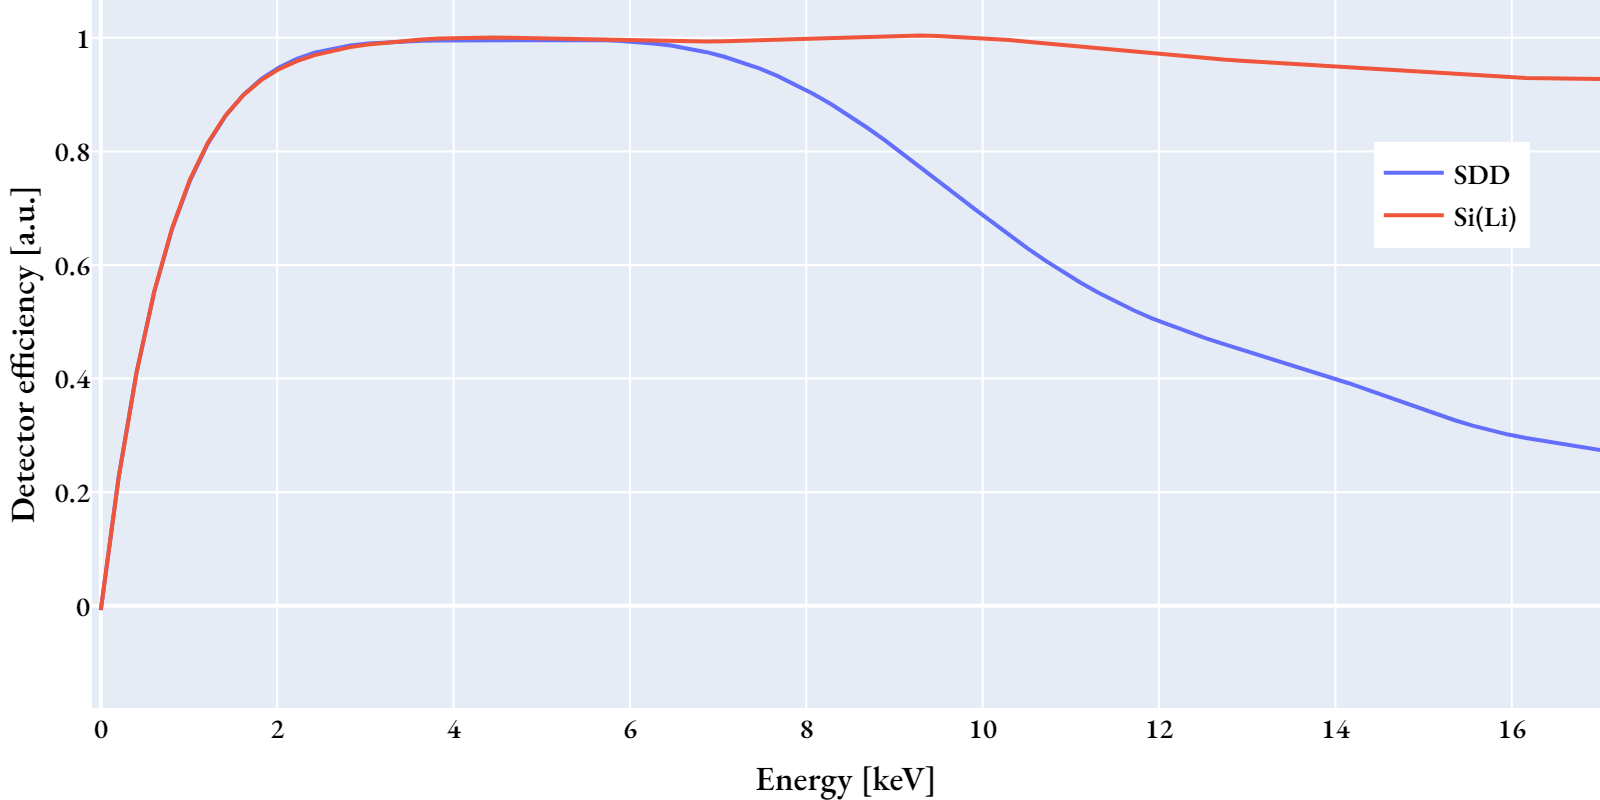
\includegraphics[width=0.8\linewidth]{figures/detector_efficiency_illustration.png}
    \caption{
        Illustration of the detector efficiency of a Si(Li) and an SDD.
        The efficiency of the SDDs decrease at higher energies because the active layer is thin, and thus high energy X-ray photons have a higher probability of passing through without creating an electron-hole pair.
        Remake of \brynjar{find one, e.g. https://www.globalsino.com/EM/page4655.html}
        \ton{Is it correct with detector efficiency at the y-axis here?}
    }
    \label{fig:detector_efficiency}
\end{figure}




% Peak broadening due to electronics


% somewhing about the controlling software, and then Vacc, Ibeam etc.?



%   - the detection system
%     - detector efficiency
%     - detector resolution
%     - dead time
%     - angle/placement of detector
%     - beam issues
%     - stray: secondary excitations in the sample
%     - Si stray
%     - holder / chamber stray detection

% figure with x,y,z, azumuthal angle, WD, etc. See DTSA-II Figure 5
% file:///C:/Users/Brynjar/Documents/Masteroppgave/potensielle%20kilder/getting-started-with-nist-dtsa-ii%20(2).pdf 




% write about geometry in EDS, feedback


% write about escape depth of different materials.
% the absorption in the sample makes the escape depth of light elements shallow. Eg. Li have an escape depth of only a few nm (Keith Thompson, Is Energy Resolution Still an Important Specification in EDS?)


% explain counts input
% explain counts output


% section "instruments" end

\clearpage

















\section{Detector status}
\label{theory:detector_status}

% \brynjar{Do not use quality control, Ton does not like it. Health check? Detector status}

The aim of this work is to improve EDS bulk quantification, and one way to do that is to make a health or status check for detectors.
A status check can both reveal errors in the setup and make the input parameters for the quantification more accurate.
Manufacturers of EDS detectors like Oxford Instruments provide a guide for how to perform quality control on their detector, but these guides focus on calibration of energy resolution and scale \cite{aztec_manual}.
As both Thompson in \cite{keith_energy_res_2013} and Goldstein in \cite{goldstein_scanning_2018} writes, the state of an EDS setup is characterized by more than its energy resolution and scale.
In 1986 Williams criticized the lack of standardized performance criteria for EDS in AEMs \brynjar{define AEM earlier}, and suggested three standardized metrics \cite{williams_standard_definitions_1986}, but these metrics were not widely adopted.
Routines for a status check seems to vary significantly between different laboratories, and the industry has not yet agreed on a standard set of metrics, aside from the energy resolution, measured by the FWHM the Mn K$\alpha$ line.
Some literature is available on status checks for TEM EDS setups, e.g. the work of Egerton and Cheng \cite{egerton_nio_characterization_1994}, updated and easily accessible in the info-sheet by Ted Pella \cite{ted_pella_nio_tem_2019}, which also sells NiO test standards.
Literature on status checks for SEM EDS setups are less common, but some papers are available and the software DTSA-II \cite{software_dtsaii} includes a quality control program, described in the textbook by Goldstein \cite{goldstein_scanning_2018}.
The similarities between EDS in SEM and TEM allow much overlap in the status checks, but there are also some differences.
One of the challenges in this work is to find the most relevant test characteristics for SEM, and especially what ranges of values should be acceptable for a healthy detector.
The value range challenge is affected by both the change from TEM to SEM and the change from the older Si(Li) detectors to the now more commonly used SDD detectors.
In this section, each of the test characteristics is described with what it is, how it is measured, and what values are acceptable.

% Mari: The tests are described by Watanabe in [30] and in the info-sheet by Ted Pella [33] which is based on the original work by R.F. Egerton and C.S. Cheng from 1994 [16].
% The complete test routine has several characteristics. Here only the most essential to this work are discussed, and an overview is found in Tab. 2.3.



\subsection{Duane-Hunt limit}
\label{theory:detector_status:duanehunt}
% put after calibration? It is done before in the code, but it is not a part of AZtec.

% What
The Duane-Hunt limit originates from a paper from Duane and Hunt in 1915 \cite{Duane_Hunt_1915}, and the Duane-Hunt limit is the maximum energy of the X-ray background radiation.
The Duane-Hunt limit is the incident beam energy, E$_0$. \brynjar{Point to E$_1$ in figure/previous theory?}
The acceleration voltage selected by the user is the nominal beam energy, while the effective beam energy is the Duane-Hunt limit, and these two values can deviate significantly.
As seen in \cref{fig:duanehunt}, the detected X-rays decline rapidly and linearly towards the nominal beam energy, but the counts does not go to zero.
It is not possible to excite X-rays above the effective beam energy, thus the spectrum should be cut off at the beam energy to allow better model fitting.
The counts above the Duane-Hunt limit are due to coincidence counts, where two X-rays are detected as one.
\brynjar{Point to where coincidence counts are explained in more detail?}
Finding the effective beam energy is done by fitting a linear function to background, where the intersection of the linear fit and the x-axis is the effective beam energy \cite{software_dtsaii} \cite[Ch. 9.1.3]{goldstein_scanning_2018}.
This solves the ambiguity of the exact beam energy, since the coincidence counts give the spectrum a tail past the effective beam energy.

% figures/Duane-Hunt.png
\begin{figure}[ht]
    \centering
    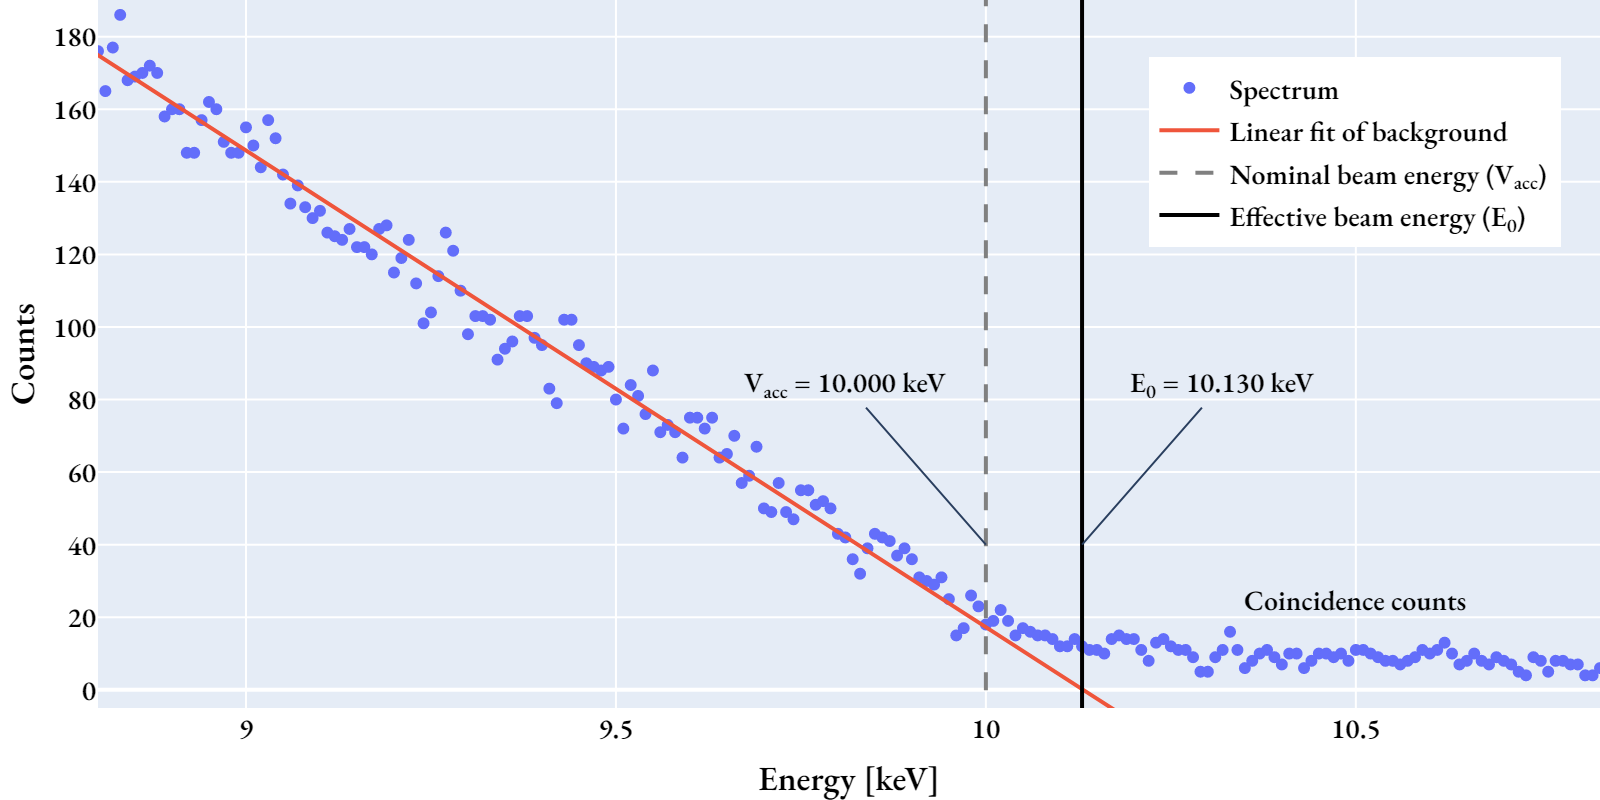
\includegraphics[width=0.8\linewidth]{figures/Duane-Hunt.png}
    \caption{
        Illustration of the Duane-Hunt limit.
        The blue dots are the X-ray counts, and the red line is a linear fit of the background.
        The gray dashed line is the nominal beam energy, and the black line is the effective beam energy.
    }
    \label{fig:duanehunt}
\end{figure}

% How
% covered above

% Acceptable values
There will be some deviation between the nominal beam energy and the effective beam energy, typically up to 0.2 keV.
Different specimen will have different deviation, due to varying conductivity.
Specimen with low conductivity will get problems with charging, which will lowers the effective beam energy.
Thus, a deviation between the nominal and effective beam energy of several kilo-electronvolts is a sign of charging \cite{dtsaii_2_manipulating_spectra}.
Charging of specimen are covered in detail in a paper by Postek and Vladár \cite{postek_charging_2015}.














\subsection{Energy resolution}
\label{theory:detector_status:energyres}


% What
The energy resolution of an EDS system is the ability to distinguish two lines at different energies, and is measured by the FWHM of the Mn K$\alpha$ peak.
The convention of using the Mn K$\alpha$ peak as the reference for the energy resolution is because of its position at 5.8987 keV, which gives an indication for both the lower and higher energies used in EDS.
The first SDD detectors had an energy resolution between 160 and 200 eV, while modern detectors can achieve energy resolution around 120 eV, which allow closer peaks to be separated \cite{keith_energy_res_2013} \brynjar{Thompson refers to Goldstein\dots}.
All EDS detectors have a stated energy resolution in its specifications, however the actual resolution of a given spectrum varies some with the acquisition settings for the same detector.
In \cite{keith_energy_res_2013} Thompson show that with the dead time kept constant, a higher input count rate gives worse resolution, with the example of 121 eV resolution with <5000 cps, and 140-150 eV resolution with >100,000 cps.
Thompson claims that EDS specifications are based on acquisition designs with low input counts.
Changes in dead time are also affecting the energy resolution, where shorter dead time give degraded resolution, because a lower dead time gives the computer shorter time to process the incoming signal and sets the channel value less accurate of each count \brynjar{Ref?}.


% Approaching the theoretical limit? Find source, Goldstein?
% TODO: amplifier noise is described with an equation in Woldseth 1973, referenced in bennett_egerton_1995.
% Woldseth 1973 figure remake in Goldstein 2003 3rd ed.: It can readily be seen that even if the noise contribution were totally eliminated, the theoretical energy resolution limit would still be greater than 100 eV for Fe Ka at 6.4 keV

% How

% Direct measurement
\brynjar{Implement check for Mn K$\alpha$ peak in the code?}
The industry standard for the energy resolution is to measure the FWHM of the Mn K$\alpha$ peak generated by an Fe$^{55}$ source, when the detector is off the microscope.
The energy resolution is not a function of the microscope, but measuring the energy resolution off the microscope negates all possible influences from the microscope, and is not a straight forward measurement to do for a user.
The most straight forward way of finding the energy resolution is to measure the FWHM of the Mn K$\alpha$ peak in a sample with Mn, preferably with high concentration as that provides a well defined peak.
The FWHM measurement should be from a Gaussian fit of the peak, because it cancels out the influence of the count statistics, as explained in \verb|\cref{eq:gaussian}| \brynjar{fix internal reference}.


% Ni Ka * 0.926
Another approach, which can be used when a sample with Ni is available, is to measure the FWHM of Ni K$\alpha$ and multiply the value with 0.926 \cite{bennett_egerton_1995}.
This approach is based on a study in 1995 where five TEM laboratories were given  standard NiO test specimen with a series of EDS test measurements to be done, where one of the tests were focused on the energy resolution.
The test used the Ni K$\alpha$ and O K$\alpha$ peaks, where the FWHM of these two lines were measured, and a linear correlation between photon energy and the square of the energy resolution was assumed.
Then the FWHM of Mn K$\alpha$ was determined by interpolation, and the factor 0.926 was reported as a sufficiently good conversion from Ni K$\alpha$ to Mn K$\alpha$ for the five TEM laboratories.
This approach is the recommended method provided by Ted Pella Inc., who manufactures standardized NiO test specimens for TEM \cite{egerton_nio_characterization_1994,ted_pella_nio_tem_2019}.


% HyperSpy
A third and more general approach, is to use the energy calibration method in HyperSpy, which estimates the FWHM of Mn K$\alpha$.
The method, \verb|EDSModel.calibrate_energy_axis()|, is available for EDS spectrum from SEM and TEM.
The method has two default arguments: \verb|calibrate='resolution'| and \verb|xray_lines='all_alpha'|.
The estimation of the FWHM of Mn K$\alpha$ is done in two steps.
The first step is to fit the width of all the lines in the spectrum, which is needed to get a correct reference peak width, i.e. an account for the peak broadening of the detector \ton{This I read from the HS code, line 50 in: \url{https://github.com/hyperspy/hyperspy/blob/842d6d9713d866960a033d4006200a43841079fe/hyperspy/models/edsmodel.py}}.
The second step utilizes an equation by Fiori and Newbury from a conference paper in 1978, and while this original paper is hard to find, the equation is included in Goldstein \cite[Ch. 16.1.1]{goldstein_scanning_2018} with a reference to the original paper.
The equation use one known line in the spectrum to estimate what the FWHM would be at an arbitrary energy, e.g. Mn K$\alpha$:
% \brynjar{original: Fiori, C. E., and Newbury, D. E. (1978). In SEM/1978/I, SEM, Inc., AFM O'Hare, Illinois, p. 401.}

\begin{equation}
    \label{eq:estimateFWHM}
    \textnormal{FWHM}(E) =  \sqrt{2.5 * (E - E_\textnormal{ref}) + \textnormal{FWHM}^2_{\textnormal{ref}}}
\end{equation}

Where $E$ is the energy of the wanted FWHM, i.e. Mn K$\alpha$ for estimating the energy resolution.
$E_\textnormal{ref}$ is the energy of a reference line in the spectrum, and $\textnormal{FWHM}_{\textnormal{ref}}$ is the FWHM of that line.
When using the HyperSpy method \verb|calibrate_energy_axis|, the user should be aware of the argument \verb|xray_lines|, which can either be a list of strings with line names or \verb|'all_alpha'|, the latter being the default value for the argument.
As of HyperSpy v1.7.3, the reference line in \cref{eq:estimateFWHM} is the first line in \verb|xray_lines|, which becomes the alphabetically first line when using \verb|'all_alpha'|.
The fact that the reference line is only the first line in the list, is not documented clearly in the HyperSpy documentation, and can yield unexpected results when the first line is not a well-defined peak.
The method works well when the reference line is a well-defined peak. \brynjar{Should probably give a definition of "well-defined" \dots}
% \brynjar{Discuss: when taking a series of spectra with different Vacc, the first line (eg AsKa in GaAs or AlKa in SU9000) is poorly defined for 10 kV and 5 kV respectively, resulting in weirdly poor Mn Ka estimate.}



% TODO: bruke average istedenfor én peak? forskjellige peaks gir forskjellige tall
% Er det best om det er user defined peak?


% Acceptable values
% TODO: run this by ton
\ton{This paragraph about acceptable values are bad. Any suggestions here?}
The energy resolution of a taken spectrum should be close to what the specifications of the EDS.
Deviations implicate \dots (High cps? Low DT? What else?)
% e.g. deviations when using the HS method implicate that the reference line is not a well-defined peak, which can be caused by ...
As explained, the theoretical limit of the FWHM of Mn K$\alpha$ is XXX \brynjar{explain above!}.
The HyperSpy method will raise an ValueError if the estimated energy resolution is below 110 eV \brynjar{line 450, \url{https://github.com/hyperspy/hyperspy/blob/842d6d9713d866960a033d4006200a43841079fe/hyperspy/models/edsmodel.py}}.




\subsection{Scale and offset}
\label{theory:detector_status:scaleoffset}
% scale and offset in one subsection?

% % What
% What is the scale and offset.
% Typical values for the scale.

% % How
% Measure two far apart peaks and find their distance in the spectrum.
% Or, use the HS function, which does \dots

% % Acceptable values
% Deviations should be \dots
% Large deviations implicate \dots


\subsection{Calibrating peak positions}
\label{theory:detector_status:peakpositions}

% % What
% What is the peak position.
% Also mention the peak width?
% Why does it deviate from the theoretical value.
% Figure of Mo K$\alpha$ peak which is not centered?
% Why bigger changes at higher energies.

% % How
% Manual: add gaussians at the expected position and fit.
% HS: adds gaussians at the expected position and fit with the centre as free parameter.

% % Acceptable values
% Deviations can be higher at higher energies, but should be \dots
% Large deviations implicate \dots


% one section on the calculated value for each line of interest?
% Line           True E [keV]   Calib. E [keV] Area [counts]  Max (fit)      Sigma [keV]    FWHM [eV]      Fiori P_10/B

\subsection{Fiori peak-to-background ratio}
\label{theory:detector_status:fiori}

% What
One of the metrics describing the quality of a spectrum is the relation between the signal in peaks and in the background, which is most commonly described by the Fiori peak-to-background ratio (P/B), at least for TEM EDS \cite{williams_carter_tem_2009}.
Some modern detectors can acquire extremely high counts per second, partly because of the larger sensor sizes, like the newest Oxford Instruments detector Ultim Max EDS with up to 170 mm$^2$, which supposedly can acquire up to 1.5 million counts per second \cite{oxford_ultim_max}.
However, having a high count rate does not necessarily mean that the spectrum yielded will have high quality, because the signal in the peaks can be very low compared to the background.
Having a metric for the ratio between the signal in peaks and in the background is therefore important both for establishing what makes a good detector, and also if an acquired spectrum have high quality.
The peak-to-background ratio in a certain detector will vary with the specimen studied and the detector settings, and can thus be used as a parameter to assess the quality of a spectrum.
The Fiori P/B was originally made for TEM and STEM, but arguments for why and how it is relevant for SEM are presented below.
The original definition of the Fiori P/B is from a publication by Fiori, Swyt, and Ellis in 1982 \cite{fiori_peak_background_1982} in \emph{Microbeam Analysis}, which is available at the NTNU library, where the definition is:

\begin{equation}
    \label{eq:fiori_pb}
    \textnormal{Fiori P/B} = \frac{\textnormal{Total counts in the peak above the background}}{\textnormal{Background counts in a 10 eV window at the peak center}} = \frac{P}{B}
\end{equation}


% Fiori and Newbury 1978: https://solo.bodleian.ox.ac.uk/permalink/f/89vilt/oxfaleph010956585 
% bestilt gjennom Oria

% https://bibsys-almaprimo.hosted.exlibrisgroup.com/permalink/f/13q4kuj/BIBSYS_ILS71489306340002201
% https://bibsys-almaprimo.hosted.exlibrisgroup.com/permalink/f/13q4kuj/BIBSYS_ILS71488306410002201

The Fiori P/B is illustrated in \cref{fig:fiori_pb}.
A paper from Zemyan and Williams in 1994 \cite{zemyan_standard_performance_1994} includes the definition and a brief discussion of why the Fiori P/B metric is superior to other P/B metrics.
A more detailed discussion on the different P/B metrics are published by Williams in \emph{Microbeam Analysis} in 1986 \cite{williams_standard_definitions_1986}.
The main advantages are the simplicity, robustness, and relevance to the generated characteristic X-ray.
The metric can be used to assess artifacts in an acquired spectrum by either comparing the metric to a reference spectrum from the same detector, or by comparing to theoretical predictions.
The robustness of the Fiori P/B comes from how the metric can be used on different detectors to compare the quality of the spectra they yield.
The metric is unaffected by different energy resolutions, as all the counts in the peak are included in the numerator, thus different peak broadening does not affect the metric.
The area of the peak is defined as the integrated counts above the background, because this was the best way to define the area of the peak in the 1970s, when the metric was first defined.
The relevance to the characteristic X-ray comes from having the denominator as a fixed 10 eV window, or approximated only one channel, which puts the metric in the same order of magnitude as if the natural line width of the peak had been used.


% TODO: arguments for why it is relevant for SEM
\brynjar{TODO: Paragraph about why this metric is relevant for SEM.}


% figures/FioriPB_TODO_remake.png
\begin{figure}
    \centering
    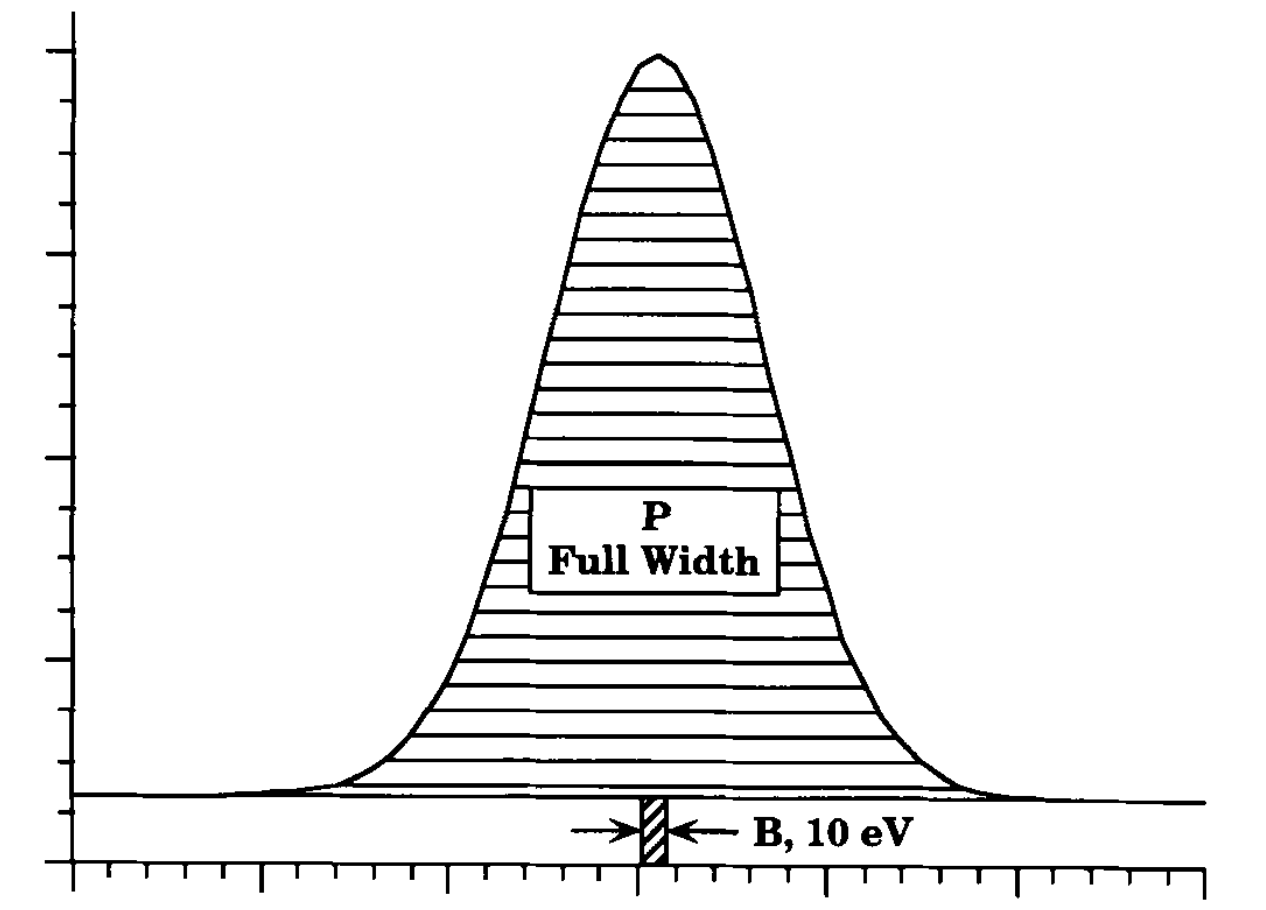
\includegraphics[width=0.6\linewidth]{figures/FioriPB_TODO_remake.png}
    \caption{Illustration of the Fiori P/B.
        P is all the counts in the actual peak, i.e. not including the background.
        B is the counts in a 10 eV window at the peak center.
        \brynjar{TODO: remake this figure.}}
    \label{fig:fiori_pb}
\end{figure}

% How (and that is the issue)
% Issue with Fiori, the calculation
Even though the definition of the Fiori P/B is simple, the actual calculation of the metric is confusingly described slightly different in different sources.
Calculating the metric the same way is critical for comparing the results on different setups.
When the metric was developed, model fitting of the spectrum was not as trivial as it is today, and thus integration windows had to be used to estimate the peak and the background.
In the 1986 paper by Williams, the background B can be calculated by peak subtraction after using library standard to do a peak fitting, or B can be calculated with the specimen used as its own standard.
Using the specimen as its own standard seems to be the common way of calculating the B, as it is the way Zemyan and Williams define B in their 1994 paper \cite{zemyan_standard_performance_1994}, with their figure reproduced in \cref{fig:fiori_pb_reality}.
The figure illustrates one of the ways to calculate the P and B: the background is estimated as the average counts in two integration windows before and after the peak divided by the number of channels, and the peak is estimated as the integrated counts minus the averaged background.
% Withouth the possibility of fitting the spectrum to a model, the method with the integration windows is the only way to calculate the Fiori P/B.
Since the use of integration windows have to be done manually, the robustness of the metric is lowered.
The user must set the integration windows so that they do not include any other minor peaks, the background windows must be close enough to the peak so that the averaged background represents the background under the peak well enough, and the integration window of the peak must include the counts in the peak, but not include counts from other peaks.
Where the peak starts and ends is a subjective choice, and will vary between users.
% Different materials
One of the sources to different integration windows is the use of different materials for the test.
The integration windows have to be adapted to the material, as some suggested test materials have other peaks close to the main peak.
The topic of choosing a test material is covered in \brynjar{TODO: internal reference to test material section, coming later.}
% Something about overlapping peaks, like in the illustration which probably have a minor peak at the left side?
The problem with subjective choice of integration window, because of the lack of an agreed test standard \cite{williams_standard_definitions_1986}, is exemplified in the EDAX Insight newsletter from September 2018 \cite{edax_insight_2018}, where they have an illustration of the Fiori P/B where the background windows are > 2 keV away from the peak, which is not in agreement with their reference.
The widths of the integration windows are also varying in different papers, which probably does not affect the results too much as the background is converted to an estimate for a 10 eV window, but it is not ideal.
In EDAX Insight a 300 eV window is used for each background area far from the peak, but the paper that they refer to uses two 500 eV window directly before and after the peak \cite{egerton_nio_characterization_1994}.
For calculation of P, the Zemyan and Williams paper from 1994 use a 700 eV window \cite{zemyan_standard_performance_1994}, and the Ted Pella info-sheet on their NiO standard sample uses a 600 eV window \cite{ted_pella_nio_tem_2019}.
This is probably a result of different materials, i.e. Cr and Ni, having different peak widths, but it is not ideal for comparison.
The inconsistency of the actual calculation of the Fiori P/B is a problem for the metric.
This problem could be solved by fitting the spectrum to a model, and using the fitted curves to calculate the P and the B.
This would make the metric truer to the original definition, and make it more robust as the users subjective opinions does not affect the calculation, and results from different materials might be more comparable.
This option is explored in this work. \ton{Ok to mention?}




% figures/FioriPB_reality_TODO_remake.png
\begin{figure}
    \centering
    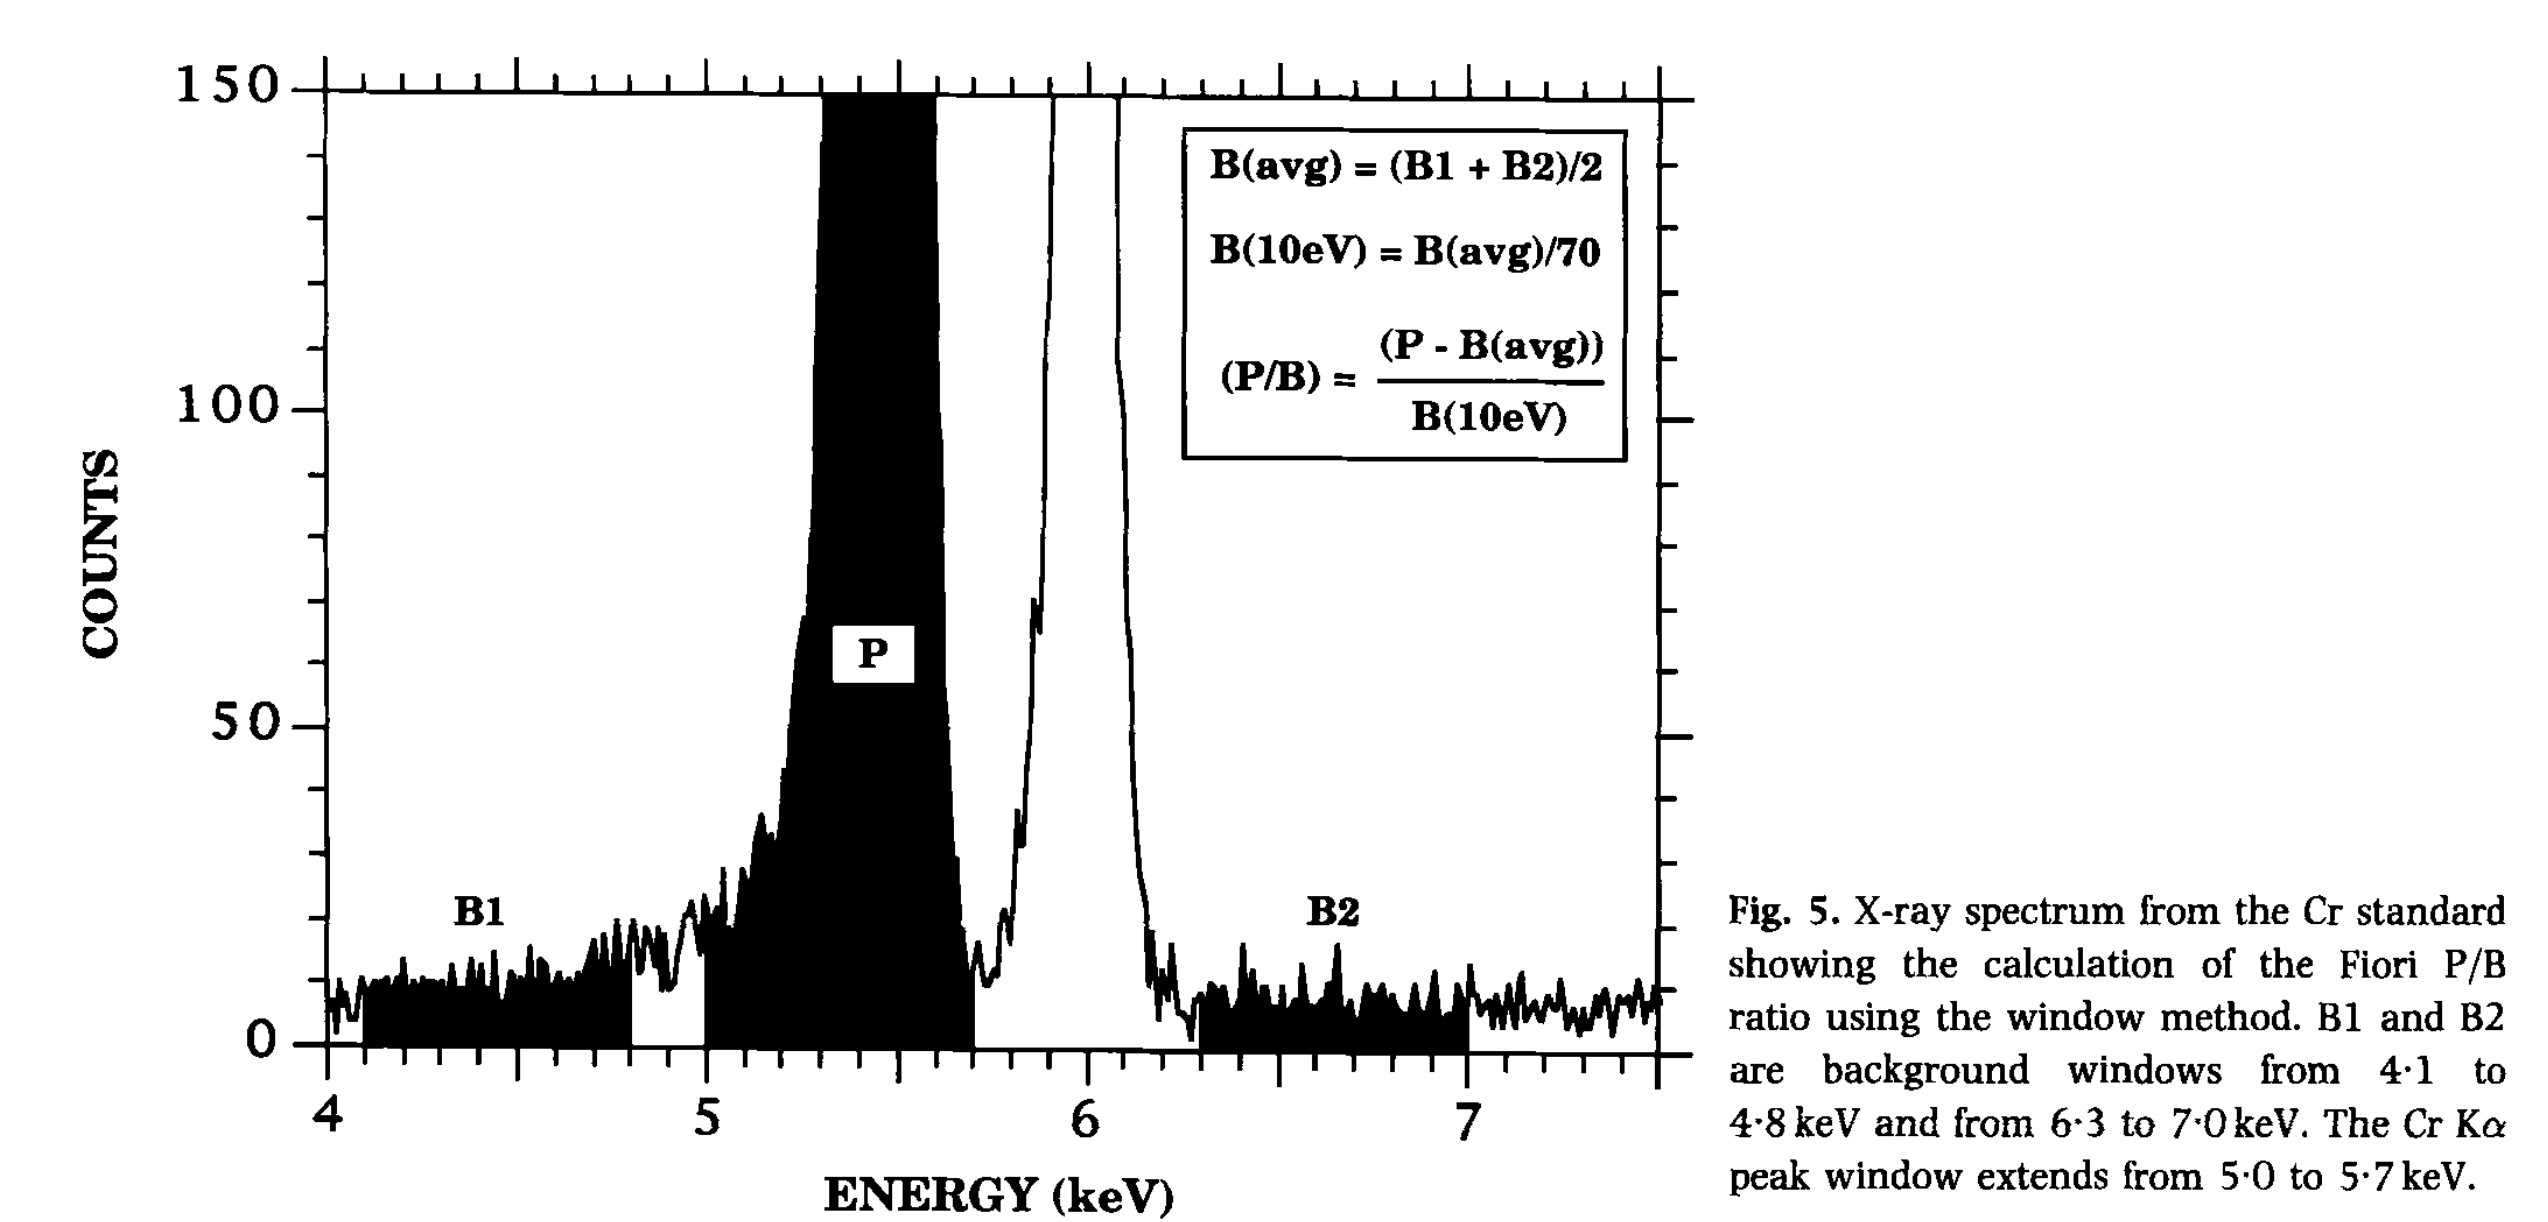
\includegraphics[width=0.6\linewidth]{figures/FioriPB_reality_TODO_remake.png}
    \caption{Illustration of how the Fiori P/B is calculated in practice.
        \brynjar{TODO: remake this figure?}
        Figure borrowed from \cite{zemyan_standard_performance_1994}.}
    \label{fig:fiori_pb_reality}
\end{figure}


% Acceptable range
There are some papers suggesting acceptable thresholds for the Fiori P/B, but they are for TEM EDS spectra.
TEM EDS signals do have lower relative background intensity than SEM EDS signals \ton{Do I need citation here?}.
This implies that a threshold should be lowered for SEM EDS signals.
Egerton and Chengs paper from 1994 \cite{egerton_nio_characterization_1994} suggests that a good TEM setup with a good signal have a Fiori P/B above 3000, while a number under 1000 indicates a bad signal.
Such high numbers might be too high for SEM EDS signals, but it is not clear what the threshold should be.
As the Fiori P/B is dividing the total area of a peak, which typically spans 20-60 channels \brynjar{right?}, while the background is only from one channel, the metric should be a high number.
It might be that the threshold should be more dependent on the detector, as detectors have a different background intensity.
However, it might be possible to use the Fiori P/B metric to optimize the settings of the detector to specific specimen, as the metric is a measure of the signal-to-noise ratio.
Higher numbers indicate a better signal-to-noise ratio, which might allow for better quantification of the specimen.
This is explored and focused on in this work, rather than trying to find a SEM threshold for the Fiori P/B.
\ton{OK to give a heads-up for the method/results here?}

% skrive hvilken jeg bruker
% skrive om de forskjellige som finnes, og hvordan de varierer. Variasjon er ikke bra from sammenlikning
% visualisere hva jeg gjør


% fra møte 5:
% det vi vil uttrykke er hvor stor andel av signalet som er nyttig. Sjekk hva Fiori skriver orginalt.
% hvor mye av signalet som er nyttig.
% varierer med %-composition
% ulik definisjon gjør at verdiene ikke kan sammenliknes. 

% EDAX: https://www.edax.com/-/media/ametekedax/files/news_events/insight_newsletter/edax-insight-vol-16-no3.pdf?la=en&revision=d212987b-0524-4056-939e-858c59d06446
% TED PELLA: file:///C:/Users/Brynjar/Documents/Masteroppgave/potensielle%20kilder/Ted%20Pella%20NiOx%20description.pdf

\subsection{Peak ratio}
\label{theory:detector_status:peakratio}
% contaminations, at least for TEM: change of Ka/La, eg in Ni
% also used for stray radiation measurements 
% stray intensity: (Ni Ka/Mo Ka) 
% stray predominent source: (Mo Ka/Mo La), only for TEM?

% the flexibility, since eg a pure Cu sample will give some statistics but not stray information.


\subsection{Peak shape}
\label{theory:detector_status:peakshape}
% The real lines are Lorentzians with width of 1-10 eV, but the peaks are wider due to electronic noise.
% Peaks are gaussians by electronic noise.
% a measure of the peak shape is the FWTM/FWHM


\subsection{Number of counts in peaks vs background}
\label{theory:detector_status:counts}

% Total counts, background counts.
% How to represent the measure better? Ratio, percentage, absolute value, etc.
% Fiori P/B is a measure already covered.


\subsection{Stray radiation measurements - when possible}
\label{theory:detector_status:stray}
% both intensity and source.
% intensity:  a major line and a stray line.
% source:  Mo Ka and Mo La ratio


\subsection{Other tests}

% linearity. nah, må ha Faraday cup
% stability
% "In a well-constructed AEM, the P/B ratio will increase with keV." (Williams and Carter, p.614)

% The two most important tests, according to Goldstein, are linearity and stability.
% requires multiple spectra of the same sample with different beam currents.
% Goldstein p. 232.






\subsection{What material to use?}

% what we want in the spectrum


%%%%%%%%%%%%%%%%%





%%%%%%%% EDS Issues
% Several issues can perturb an EDS spectrum, including peak broadening, peak distortion, silicon x-ray escape peaks, absorption edges, and the silicon internal fluorescence peak. In addition, several hardware-related problems, such as pulse pileup rejection by the main amplifier, acoustic coupling on the co-axial connector between the detector and the amplifier, ground loops, and ice in the detector system, can occur.
% https://www.semitracks.com/reference-material/failure-and-yield-analysis/failure-analysis-materials-characterization/energy-dispersive-x-ray-spectrometry.php#:~:text=History,used%20for%20x%2Dray%20characterization.





% OBS: efficiency of the detector is important